\section*{Лекция 2}
\subsection{Виды ошибок и неопределенное поведение (UB)}

C++~--- компилируюемый язык. Поговорим о том, какие ошибки бывают ошибки при компиляции и после нее.


Программа бывает некорректна по многим причинам. 
Рассмотрим ошибку компиляции \textbf{CE} Compilation Error.

Ошибки компиляции бывают разные. Например, если где-то забыть поставить точку с запятой,
то это будет \textbf{синтаксическая ошибка}. Она случается когда компилятор не смог распарсить то что написано из-за синтаксиса.
Ошибкой компиляции также считается использование переменной или функции, которые не были объявлены. 

При написании
\begin{minted}{cpp}
#include <iostream>    
\end{minted}

Мы вставляем в исходный код содержание заголовочного файла, в данном случае \underline{iostream}, 
в котором содержатся объявления функций \underline{std::cin} и \underline{std::cout}.

И если забыть подключить заголовочный файл и воспользоваться функцией, то это будет \underline{CE}.

Ошибкой будет и повторное объявление переменной в одной и той же области видимости.
\begin{minted}{cpp}
int main() {
    int x;
    int x;
}
\end{minted}

Поэтому подобный код тоже будет выдавать ошибку \underline{CE} при попытке компиляции.

Также при обычных обстоятельствах недопустимо пользоваться переменной/функцией до объявления.

\begin{minted}{cpp}
#include <iostream>

int main() {
    std::cout << x << '\n';
    int x;
}
\end{minted}
Выдаст \underline{CE} при попытке компиляции.


В целом ошибки компиляции можно разбить на три группы:
\begin{itemize}
    \item Лексические ошибки
    \item Синтаксические ошибки
    \item Семантические ошибки
\end{itemize}

Компиляция это очень сложный процесс, который состоит из разных стадий, поговорим о трех.
Так, в начале происходит лексический разбор, потом синтаксический, а потом компилятор разбирается в семантике того что написано.

Разберем поподробнее. При лексическом разборе компилятор пытается разбить код на осмысленные последовательности символов~--- \textbf{токены}.
Пример:
\begin{minted}{cpp}
    std::cout << x;
\end{minted}

Этот код будет разбиваться на токены следущим образом:
\[(std) (::) (cout) (<<) (x) (;).\]
Здесь круглыми скобками обозначены токены, на которые разберется код при лексическом разборе.

Возникает вопрос, почему компилятор определил (<<) а не например как два знака меньше (<)(<)?
На самом деле действует следущее правило. Компилятор будет идти слева направо и пока это осмысленно он будет добавлять символы к токену.
Именно поэтому не получится разбиения (std:), поскольку это неосмыслленно, а вот (std)~--- осмысленно.

Если компилятору не удалось разбить код на токены на этапе лексического разбора, то такая ошибка будет называться \textbf{лексической}.

\begin{minted}{cpp}
#include <iostream>

int main() {

    \\\\\;

    int x;
    std::cin >> x;
    std::cout << x + 5;
}
\end{minted}

При компиляции кода можно увидеть следущее, рисунок \ref{l2img1}.

\begin{figure}[h]
    \centering
    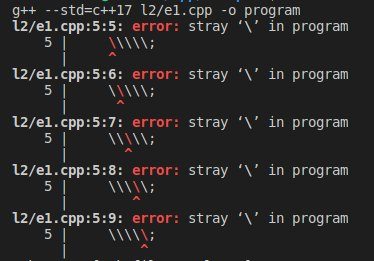
\includegraphics[width=1\textwidth]{l2img1.png}
    \caption{Пример лексической ошибки.}
    \label{l2img1}
\end{figure}

Здесь stray можно перевести как "заблудший" или "заплутавший". Компилятор не смог это как-то интерпетировать.

Приведем более подробные примеры синтаксических ошибок.

\begin{minted}{cpp}
#include <iostream>

int main() {
    int x
    std::cin >> x;
    std::cout << x + 5;
}
\end{minted}

\begin{figure}[h]
    \centering
    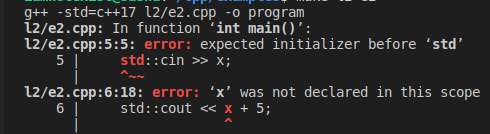
\includegraphics[width=1\textwidth]{l2img2.png}
    \caption{Пример синтаксической ошибки 1.}
    \label{l2img2}
\end{figure}

На рисунке \ref{l2img2} написано, что компилятор ожидал инициализацию перед std.
Иначе говоря он парсит строки 5 и 6 как одно выражение, так как в строке пять нет ';',
однако после объявления переменной компилятор ожидает либо ничего, либо ее инициализацию,
а так как дальнейшее инициализацией никак не является, то это ошибка. Так как эта ошибка возникла из-за  отсуствия ';' 
и была обнаружена на этапе синтаксического разбора она считается синтаксической.

Далее компиляция не прервалась и было обнаружено, что переменная \underline{x} не была объявлена, поскольку предыдущее выражение ошибочно.
Стоит отметить, что компилятор не сказал об использовании необъявленной переменной в 5-ой строке после \underline{std::cin}, так как уже отловил в этом выражении синтаксическую ошибку.
Выражения не всегда рассматриваются на предмет ошибок до конца, да и здесь это не требуется.

\begin{minted}{cpp}
#include <iostream>

int main() {
    int x;
    std::cin >> x;
    std::cout << x + 5;
    x + 5 + ;
}
\end{minted}

\begin{figure}[h]
    \centering
    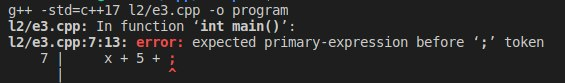
\includegraphics[width=1.3\textwidth]{l2img3.png}
    \caption{Пример синтаксической ошибки 2.}
    \label{l2img3}
\end{figure}

Поскольку '+' здесь используется как бинарный оператор, а после стоит ';', то перед ';' ожидается
некое \underline{primary-expression}, о котором будет рассказано позже.

Компилятор старается не завершать компеляцию, чтобы выдать как можно больше ошибок сразу, однако у него не всегда это получается.
Ошибки, при которых компиляция останавливается, называются \textbf{фатальными}.

\begin{minted}{cpp}
#include <iostream>
#include <aaaaaaaa>

int main() {

}
\end{minted}

\begin{figure}[h]
    \centering
    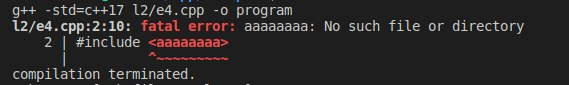
\includegraphics[width=1.3\textwidth]{l2img4.png}
    \caption{Пример синтаксической ошибки 3. Фатальная ошибка.}
    \label{l2img4}
\end{figure}

Примером фатальной ошибки будет являться подключение файла, которого не существует.

Можно привести такой неформальный пример синтаксической ошибки
\begin{center}
Я пошел лес грибы.
\end{center}
Вроде и все понятно, но синтаксически неверно.

А вот какой пример можно привести для семантической ошибки
\begin{center}
Я ем стол.
\end{center}
С точки зрения синтаксиса здесь все верно, однако есть стол это как-то странно.
Иначе говоря мы понимаем, какую пищу может есть человек, а какую нет. Человек не может есть стол.
Подобная ошибка называется семантической.

Другими словами если мы пытаемся совершить что-то невозможное, то это \textbf{семантическая ошибка}.

\begin{minted}{cpp}
#include <iostream>

int main() {
    int x;
    std::cin >> x;
    std::cout << x.size();
}
\end{minted}

\begin{figure}[h]
    \centering
    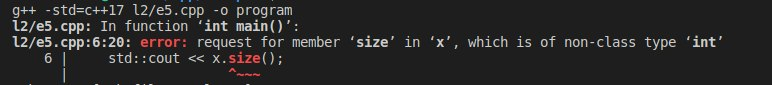
\includegraphics[width=1.3\textwidth]{l2img5.png}
    \caption{Пример семантической ошибки 1.}
    \label{l2img5}
\end{figure}

Мы пытаемся применить метод \underline{.size()} к переменной целочисленного типа,
однако это невозможно, поскольку переменная целочисленного типа не обладает методом \underline{.size()}.
О методах мы узнаем позже.

\begin{minted}{cpp}
int main() {
    int x;
    int a;
    int b;
    x++ = a + b;
}
\end{minted}

\begin{figure}[h]
    \centering
    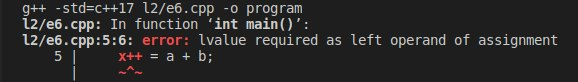
\includegraphics[width=1.3\textwidth]{l2img6.png}
    \caption{Пример семантической ошибки 2.}
    \label{l2img6}
\end{figure}

Это тоже семантическая ошибка, поскольку тому, что стоит слева от '='
невозможно присвоить что-либо, так как то что слева не является \underline{lvalue}.
О том что такое \underline{lvalue} мы тоже поговорим позднее.

Заметим, что на рисунке \ref{l2img2} также показана семантическая ошибка, так как мы пытаемся использовать необъявленную переменную.
\begin{minted}{cpp}
    int main() {
        int x;
        int x;
    }
\end{minted}

\begin{figure}[h]
    \centering
    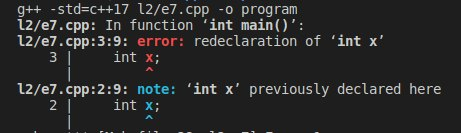
\includegraphics[width=1.3\textwidth]{l2img7.png}
    \caption{Пример семантической ошибки 3.}
    \label{l2img7}
\end{figure}

Вспомним о повторном объявлении переменной. Это тоже семантическая ошибка, рисунок \ref{l2img7}.

Также иногда семантическая ошибка возникает при неоднозначном обращении, рисунок \ref{l2img8}.

\begin{minted}{cpp}
#include <iostream>

namespace N {
    int x;
}

using namespace N;

int x = 0;

int main() {
    std::cin >> x;
    std::cout << x + 5;
}
\end{minted}

\begin{figure}[h]
    \centering
    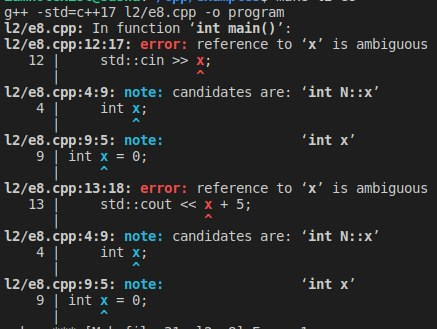
\includegraphics[width=1\textwidth]{l2img8.png}
    \caption{Пример семантической ошибки 4.}
    \label{l2img8}
\end{figure}

Здесь переменная 'x' объявлена в \underline{пространстве имен} 'N', а далее, строкой

\begin{minted}{cpp}
using namespace N;
\end{minted}

сливается с глобальной областью видимости.

Так как переменные объявлены в разных областях видимости здесь нет ошибки повторного объявления,
значит это две разные переменные. Однако после сливания не понятно, к какой именно переменной идет обращение.


Помимо ошибок компиляции существуют ошибки, которые возникают во время исполнения программы.
Они называются \textbf{Runtime error} (\textbf{RE}).